\documentclass[10pt,usenames,dvipsnames]{beamer}
\usetheme{CambridgeUS}
%\usetheme{Boadilla}
\definecolor{myred}{RGB}{163,0,0}
%\usecolortheme[named=`blue]{structure}
\usecolortheme{dove}
\usefonttheme[]{professionalfonts}
\usepackage[english]{babel}
\usepackage{amsmath,amsfonts,amssymb}
\usepackage{xcolor}
\usepackage{tikz}
\usepackage{pgfplots}
\pgfplotsset{compat=newest,compat/show suggested version=false}
\usetikzlibrary{arrows,shapes,calc,backgrounds}
\usepackage{bm}
\usepackage{textcomp}
\usepackage{gensymb}
\usepackage{verbatim}
\usepackage{paratype}
\usepackage{mathpazo}
\usepackage{listings}
\usepackage{csvsimple}

\newcommand{\cov}{\mathsf{cov}}
\newcommand{\corr}{\mathsf{corr}}
\newcommand{\var}{\mathsf{Var}}
\newcommand{\plim}{\mathrm{plim\ }}
\newcommand{\E}{\mathsf{E}}
\newcommand{\Est}{\mathsf{Est.Var}}
\newcommand{\Asy}{\mathsf{Asy.Var}}
\newcommand{\Esta}{\mathsf{Est.Asy.Var}}
\newcommand{\tr}{\mathrm{tr}}
\newcommand{\Prob}{\mathrm{Prob}}
\newcommand{\Med}{\mathsf{Med}}
\newcommand{\rank}{\mathsf{rank}}
\newcommand{\argmin}{\mathsf{arg\,min}}

\newcommand{\cc}[1]{\texttt{\textcolor{blue}{#1}}}

\definecolor{ttcolor}{RGB}{0,0,1}%{RGB}{163,0,0}

% Number theorem environments
\setbeamertemplate{theorem}[ams style]
\setbeamertemplate{theorems}[numbered]

% Reset theorem-like environments so that each is numbered separately
\usepackage{etoolbox}
\undef{\definition}
\theoremstyle{definition}
\newtheorem{definition}{\translate{Definition}}

\definecolor{ttcolor}{RGB}{0,0,1}%{RGB}{163,0,0}
\definecolor{mygray}{RGB}{248,249,250}

% Change colours for theorem-like environments
\definecolor{mygreen1}{RGB}{0,96,0}
\definecolor{mygreen2}{RGB}{229,239,229}
\setbeamercolor{block title}{fg=white,bg=mygreen1}
\setbeamercolor{block body}{fg=black,bg=mygreen2}

\lstdefinestyle{numbers}{numbers=left, stepnumber=1, numberstyle=\tiny, numbersep=10pt}
\lstdefinestyle{MyFrame}{backgroundcolor=\color{yellow},frame=shadowbox}

\lstdefinestyle{rstyle}%
{language=R,
	basicstyle=\footnotesize\ttfamily,
	backgroundcolor = \color{mygray},
	commentstyle=\slshape\color{green!50!black},
	keywordstyle=\bfseries\color{blue!50!black},
	identifierstyle=\color{blue},
	stringstyle=\color{orange},
	%escapechar=\#,
	rulecolor = \color{mygray}, 
	showstringspaces = false,
	showtabs = false,
	tabsize = 2,
	emphstyle=\color{red},
	frame = single} 

\setbeamertemplate{navigation symbols}{}

\lstset{language=R,frame=single}

\AtBeginSection{\frame{\sectionpage}}

% Remove Section 1, Section 2, etc. as titles in section pages
\defbeamertemplate{section page}{mine}[1][]{%
	\begin{centering}
		{\usebeamerfont{section name}\usebeamercolor[fg]{section name}#1}
		\vskip1em\par
		\begin{beamercolorbox}[sep=12pt,center]{part title}
			\usebeamerfont{section title}\insertsection\par
		\end{beamercolorbox}
	\end{centering}
} 

\setbeamertemplate{section page}[mine]  

\hypersetup{colorlinks, urlcolor=blue, linkcolor = myred} 

\title{R406: Applied Economic Modelling with Python}
\subtitle{\textcolor{myred}{First-order Difference Equations}}
\author[Kaloyan Ganev,  Andrey Vassilev]{Kaloyan Ganev (main author) \\
Andrey Vassilev (minor modifications)}

\date{} 

\begin{document}
\maketitle

\begin{frame}[fragile]
\frametitle{Lecture Contents}
\tableofcontents
\end{frame}

\section{Introduction}
\subsection{Definition of Concepts}
\begin{frame}[fragile]
\frametitle{Discrete Time}
\begin{itemize}
%	\item Differential equations describe economic dynamics in continuous time
%	\item Derivatives measuring instantaneous rates of change, accelerations, decelerations, etc., are used in them
	\item In many cases a variable of interest can be determined from its past values (as well as potentially other quantities)
	\item Examples
		\begin{itemize}
		\item The end-period balance of a bank account can be computed from the starting balance plus deposits/withdrawals and interest
		\item The stock of capital at a point in time is determined by the stock from the previous period, investment and depreciation
		\end{itemize}
	\item Here we consider the case of discrete time: $t$ takes only integer values:
	\[
		t = \ldots, -3, -2, -1, 0, 1, 2, 3,\ldots
	\]
%	\item Changes of variables are no longer instantaneous, so derivatives are not adequate in the description of dynamics
%	\item The notion of differences is much more appropriate, therefore the term \textcolor{red}{\emph{difference equations}}
\end{itemize}
\end{frame}

%\begin{frame}[fragile]
%\frametitle{A Word on Notation}
%\begin{itemize}
%	\item The integer values that the time variable takes serve to index economic variables 
%	\item Each different value indexes a separate period for which information on the respective economic variable is recorded
%	\item We make a slight change of notation from differential equations so that we take into account the above
%	\item Instead of writing:
%	\[
%		\dot{y}(t)
%	\]
%	to describe the (instantaneous) change of $x$, here we write:
%	\[
%		\textcolor{red}{\Delta y_{t}}\quad ( = y_{t} - y_{t-1})
%	\]
%	to describe the change of $x$ between two consecutive periods (or, the per-unit-of-time change)
%\end{itemize}
%\end{frame}
%
%\begin{frame}[fragile]
%\frametitle{A Word on Notation (2)}
%\begin{itemize}
%	\item Analogies to higher-order derivatives are easily made
%	\item For example, the second derivative of $x$ (in the continuous case), $\ddot{x}(t)$, is matched by:
%	\[
%		\Delta^{2}y_{t} = \Delta y_{t} - \Delta y_{t-1}
%	\]
%	\item The latter is also interpreted as acceleration
%	\item The same line of reasoning is then further extended to third differences, fourth differences, etc.
%\end{itemize}
%\end{frame}

\begin{frame}[fragile]
	\frametitle{What Are Difference Equations?}
	\begin{itemize}
		\item In general a difference equation can be stated as a function relating the variable to its own past values
		\item Formally written,
		\[
		y_{t+1} = f(y_{t},y_{t-1},\ldots)
		\]
		\item We call this a \emph{recursive relationship}
		\item Every next value is obtained from this relationship; for example, in the relationship $y_{t+1} = f(y_{t})$:
		\[
		y_{t+2} = f(y_{t+1}) = f(f(y_{t})) = f^{2}(y_{t})
		\]
		\item From this follows:
		\[
		y_{t+k} = f^{k}(y_{t})
		\]
		
		\textcolor{orange}{Note: }\textcolor{magenta}{$k$ is not interpreted as a power!}
		
	\end{itemize}
\end{frame}

%\begin{frame}[fragile]
%\frametitle{What Are Difference Equations?}
%\begin{itemize}
%	\item By analogy to differential equations (where derivatives are included), difference equations are equations in which differences of variables are included
%	\item The order of differences defines the order of equations
%	\item Examples:
%	\[
%		\begin{array}{lcl}
%			\Delta y_{t} = 8,\\
%			\Delta y_{t} = 0.4y_{t} + 2t + 3
%		\end{array}
%	\]
%	are first-order difference equations, while
%	\[
%		\begin{array}{lcl}
%			\Delta^{2}y_{t} = 0.5y_{t} - 11y_{t-1}
%		\end{array}
%	\]
%	is a second-order difference equation
%\end{itemize}
%\end{frame}
%
%\begin{frame}[fragile]
%\frametitle{What Are Difference Equations? (2)}
%\begin{itemize}
%	\item Take, for example, the equation:
%	\[
%		\Delta y_{t+1} = 0.6y_{t} - 21
%	\]
%	and recall the definition of differences (through deltas)
%	\item If we leave on the left-hand side the variable with the largest index, and move all the rest to the right-hand side, we have:
%	\[
%		y_{t+1} =  1.6y_{t} - 21
%	\]
%	\item This shows that the value at time $(t+1)$ can be thought of as a function of the value at time $t$ (and possibly some other stuff, such as time independently, or another variable)
%\end{itemize}
%\end{frame}

\begin{frame}[fragile]
	\frametitle{What Are Difference Equations? (2)}
	\begin{itemize}
		\item Sometimes difference equations are written in more general, \textbf{implicit} form as \[ F(y_{t+1},y_t,y_{t-1},\ldots)=0. \]
		We shall ignore such cases and work with \textbf{explicit} difference equations, i.e. ones that can be solved for the variable with the largest index
		\item The order of a difference equation is given by the difference between the largest and the smallest time indexes
		\item For example, the equation
		\[ y_{t+1} = f(y_t, y_{t-1}, y_{t-2}) \]
		is a third-order equation because $(t+1) - (t-2) = 3$
	\end{itemize}
\end{frame}

\begin{frame}[fragile]
	\frametitle{What Are Difference Equations? (3)}
	\begin{itemize}
		\item A difference equation, e.g. \[ y_{t+1} = f(y_t), \] 
		can be re-written as 
		\[ y_{t+1} - y_t = f(y_t) - y_t. \] 
		\item We can define the (first) difference as $ \Delta y_{t} := y_{t} - y_{t-1} $
	and a new right-hand side $ g(y):= f(y)-y$
		\item The above equation can then be written as 
		\[ \Delta y_{t+1} = g(y_t), \]
		hence the name \textit{difference equation}
		\item While you may not see immediate benefits from writing the equation to feature an explicit difference operator $ \Delta $, this form becomes useful to motivate the transition to differential equations
	\end{itemize}
\end{frame}


\subsection{Classification}
\begin{frame}[fragile]
\frametitle{Linear vs. Non-linear Equations}
\begin{itemize}
	\item Recursive relationships can be either \textcolor{blue}{linear} or \textcolor{red}{non-linear}
	\item Therefore linear and non-linear difference equations
	\item \textcolor{orange}{(Note again that time and/or other variables could also appear as function arguments)}
	\item We will stick most of the time to linear equations
	\item Linearity will be directly assumed, while non-linearity will be explicitly indicated when necessary 
\end{itemize}
\end{frame}

\begin{frame}[fragile]
\frametitle{Constant-coefficients vs. Variable-coefficients Equations}
\begin{itemize}
	\item Take the equation: 
	\[
		y_{t+3} = ay_{t+2} + by_{t+1} + cy_{t} + d
	\]
	where $a,b,c,d$ are constants

	This is a \textcolor{blue}{constant-coefficients difference equation}
	
	\item Compare this to: 
	\[
		y_{t+3} = a_{t+2}y_{t+2} + b_{t+1}y_{t+1} + c_{t}y_{t} + d_{t}
	\]
	This is a \textcolor{red}{variable-coefficients difference equation}
\end{itemize}
\end{frame}

\begin{frame}[fragile]
\frametitle{Autonomous vs. Non-autonomous Difference Equations}
\begin{itemize}
	\item \textcolor{blue}{Autonomous} (or time-invariant) equations: time does not enter independently as an argument of $f(\cdot)$; example:
	\[
		y_{t} = 0.4y_{t-1} + 2
	\]
	\item \textcolor{red}{Non-autonomous} (or time-variant) equations: time enters independently as an argument:
	\[
		y_{t} = 0.4y_{t-1} + 3t + 2
	\]
	\item The latter are much more difficult to study, and we will only occasionally mention them
\end{itemize}
\end{frame}

\begin{frame}[fragile]
\frametitle{Homogeneous vs. Non-homogeneous Equations}
\begin{itemize}
	\item Take the following equation where all instances of the $y$ variable are on the left-hand side, and `all the rest' is summarized on the right-hand side in $g(t)$:
	\[
		y_{t+2} + ay_{t+1} + by_{t} = g(t)
	\]
	\item \textcolor{orange}{(A second-order equation in this case, but order here does not matter)}
	\item If $g(t) = 0$, the equation is \textcolor{blue}{homogeneous}\footnote{For such equations, if $y_{t}$ is a solution, so is $\alpha y_{t}$.}
	\item If $g(t) \neq 0$, the equation is \textcolor{red}{non-homogeneous}
\end{itemize}
\end{frame}

\section{The Initial-value Problem}
\begin{frame}[fragile]
\frametitle{The Initial-value Problem}
\begin{itemize}
	\item Take the equation:
	\[
		y_{t} = f(y_{t-1}, y_{t-2},\ldots,y_{t-p})
	\]
	\item In order to be able to solve for $y_{t}$, $p$ starting values will be needed
	\item Otherwise it would be impossible to find the solution
	\item In the case of the first-order equation, one such value is needed
\end{itemize}
\end{frame}

\section{Equilibrium and Stability Conditions}
\begin{frame}[fragile]
\frametitle{Equilibrium}

\begin{itemize}
	\item We begin with the autonomous first-order-equation case so that the idea is grasped more easily
	\item We will consider stability conditions again when we get to higher-order equations
	\item Start from the definition of a function's fixed point:
\end{itemize}

\begin{definition}
Let $K \subset \mathbb{R}^{n}$ and let $\mathbf{f}$ be a function that maps $\mathbf{x} \in K$ into another point $\mathbf{f}(\mathbf{x})\in K$ (i.e. the function maps $K$ into itself). If the point $\mathbf{x}^{*}$ is such that $\mathbf{f}(\mathbf{x}^{*}) = \mathbf{x}^{*}$, then $\mathbf{x}^{*}$ is called a \textbf{fixed (or equilibrium) point}.
\end{definition}

\end{frame}

\begin{frame}[fragile]
\frametitle{Equilibrium (2)}
\begin{itemize}
	\item In the current context $K$ consists of all $y_{t}$'s
	\item For example, in the difference equation $y_{t+1} = f(y_{t})$, $f$ maps $y_{t}$ into $y_{t+1}$
	\item The definition then implies that $y^{*}$ is an equilibrium point if and only if (iff):
	\[
		y^{*} = f(y^{*})
	\]
	\item Graphically, this means that equilibrium points always lie on the 45\degree\ line
	\item \textcolor{orange}{Example:} Find the equilibrium points of $f(x) = x^{3}$; make a graphical sketch of your solution
\end{itemize}
\end{frame}

\begin{frame}[fragile]
\frametitle{Stability of Equilibrium}
Let $y^{*}$ be an equilibrium point of $f$. Some definitions follow.
\begin{definition}
	The point $y^{*}$ is \textbf{stable} if for any $\varepsilon > 0\,\exists\, \delta > 0$:
\[
	|y_{0} - y^{*}| < \delta \Rightarrow |f^{n}(y_{0}) - y^{*}| < \varepsilon, \, \forall n > 0.
\]

Otherwise, $y^{*}$ is \textbf{unstable}.
\end{definition}

\begin{definition}
	The point $y^{*}$ is \textbf{repelling} if $\exists\,\varepsilon > 0$:
\[
	0 < |y_{0} - y^{*}| < \varepsilon \Rightarrow |f(y_{0}) - y^{*}| > |y_{0} - y^{*}|.
\]
\end{definition}
\end{frame}

\begin{frame}[fragile]
\frametitle{Stability of Equilibrium (2)}
\begin{definition}
	The point $y^{*}$ is \textbf{attracting (asymptotically stable)} if:
	\begin{enumerate}
		\item It is stable
		\item $\exists\,\eta > 0$:
		\[
			|y_{0} - y^{*}| < \eta \Rightarrow \lim_{t\to\infty}y_{t} = y^{*}.
		\]
		If $\eta = \infty$, then $y^{*}$ is \textbf{globally asymptotically stable}.
	\end{enumerate}		 
\end{definition}
\end{frame}

\begin{frame}[fragile]
\frametitle{Stability of Equilibrium (3)}

\begin{theorem}
Let $y^{*}$ be a fixed point of $y_{t+1} = f(y_{t})$, and let $f$ be continuously differentiable at $y^{*}$. Then:
\begin{enumerate}
	\item If $|f'(y^{*})| < 1$, then $y^{*}$ is an attractor
	\item If $|f'(y^{*})| > 1$, then $y^{*}$ is a repeller
	\item If $|f'(y^{*})| = 1$ and:
	\begin{enumerate}
		\item if $f''(y^{*}) \neq 0$, then $y^{*}$ is unstable
		\item if $f''(y^{*}) = 0$ and if $f'''(y^{*}) > 0$, then $y^{*}$ is unstable
		\item if $f''(y^{*}) = 0$ and if $f'''(y^{*}) < 0$, then $y^{*}$ is an attractor
	\end{enumerate}
	\item If $f'(y^{*}) = -1$ and:
	\begin{enumerate}
		\item if $-2f'''(y^{*}) - 3[f''(y^{*})]^{2} < 0$, then $y^{*}$ is an attractor
		\item if $-2f'''(y^{*}) - 3[f''(y^{*})]^{2} > 0$, then $y^{*}$ is unstable
	\end{enumerate}
\end{enumerate}
\end{theorem}

\textcolor{orange}{Note:} \textcolor{magenta}{Theorems are provided just for usage and reference, no proofs are given or required!}

\end{frame}

\begin{frame}[fragile]
\frametitle{Stability of Equilibrium (4)}
\begin{itemize}
	\item There exist fixed points which are neither attractors not repellers
	\item Take for example:
	\[
		y_{t+1} = -y_{t} + k
	\]
	\item If $y_{0}$ is the initial value, then
	\[
		\begin{array}{lcl}
			y_{0} = y_{2} = y_{4} = \ldots\\
			y_{1} = y_{3} = y_{5} = \ldots
		\end{array}
	\]
	\item Although there is a fixed point $y^{*} = \displaystyle \frac{k}{2}$, if $y_{0} \neq y^{*}$, the system cycles between $y_{0}$ and $-y_{0} + k$ without getting nearer or farther from the fixed point over time
\end{itemize}
\end{frame}

\begin{frame}[fragile]
\frametitle{Stability of Equilibrium (5)}
\begin{itemize}
	\item A solution $y_{n}$ is periodic if 
	\[
		y_{n+m} = y_{n}
	\]
	for some fixed integer $m$ and all $n$. The smallest integer $m$ is called the \textbf{the period of the solution}.
\end{itemize}
\begin{definition}
	If the sequence $\{y_{t}\}$ has $q$ repeating values, then $y_{1}, y_{2},\ldots, y_{q}$ are called \textbf{period points}, and the set $\{y_{1},y_{2},\ldots,y_{q}\}$ is called a \textbf{periodic orbit}.
\end{definition}

\begin{itemize}
	\item For example, if the equation is $y_{t+1} = f(y_{t})$, a $k$-periodic point is the $y$-coordinate of the intersection point of $f^{k}(y)$ and the 45\degree-line $y_{t+1} = y_{t}$
\end{itemize}

\end{frame}

\begin{frame}[fragile]
\frametitle{Stability of Equilibrium (6)}
\begin{theorem}
	Let $b$ be a $k$-period point of $f$. Then $b$ is:
	\begin{enumerate}
		\item Stable if it is a stable fixed point of $f^{k}$
		\item Asymptotically stable if it is an attracting point of $f^{k}$
		\item Repelling if it is a repelling fixed point of $f^{k}$
	\end{enumerate}
\end{theorem}
\end{frame}


\section{First-order Difference Equations}
\subsection{Problem Setup}
\begin{frame}[fragile]
\frametitle{First-order Difference Equations: Problem Setup}
\begin{itemize}
	\item A first-order difference equation is one in which the recursive relationship extends only to one period in the past, i.e.:
	\[
		y_{t+1} = f(y_{t})
	\]
	\item Initial-value problem:
	\[
		\left|
		\begin{array}{lcl}
			y_{t+1} = f(y_{t})\\
			y(0) = y_{0}
		\end{array}
		\right.
	\]
	where $y_{0}$ is given initially
	\item It is easy to see that $y_{1} = f(y_{0}),\, y_{2} = f(y_{1}),\, y_{3} = f(y_{2})$, etc.
	\item In other words, it implies the following sequence of values:
	\[
		y_{0}, f(y_{0}), f(f(y_{0})), f(f(f(y_{0})),\ldots
	\]
	\item As already noted, sometimes this is denoted more conveniently as follows:
	\[
		y_{0}, f(y_{0}), f^{2}(y_{0}), f^{3}(y_{0}),\ldots
	\]
\end{itemize}
\end{frame}

\subsection{Solution}
\begin{frame}[fragile]
\frametitle{Solution}
\begin{itemize}
	\item Start with the linear non-homogeneous, constant-coefficients case:
	\[
		\left|
		\begin{array}{lcl}
			y_{t+1} = ay_{t} + b\\
			y(0) = y_{0}
		\end{array}
		\right.
	\]
	\item Beginning with $y_{0}$, the next values are obtained through iteration:
	\[
		\begin{array}{lcl}
			y_{0}\\
			y_{1} = ay_{0} + b\\
			y_{2} = ay_{1} + b = a^{2}y_{0} + ab + b\\
			\ldots\\
			y_{t} = a^{t}y_{0} + b(a^{t-1} + a^{t-2} + \ldots + a + 1)
		\end{array}
	\]
\end{itemize}
\end{frame}

\begin{frame}[fragile]
\frametitle{Solution (2)}
\begin{itemize}
	\item We have the sum of a geometric series in the parentheses
	\item Using the standard formula, this sum equals:
	\[
	\left\{
	\begin{array}{lcl}
			 \displaystyle \frac{1 - a^{t}}{1-a},\quad a\neq 1\\
			 \quad\\
			 t, \quad a = 1 
	\end{array}
	\right.
	\]
	\item Let $a\neq 1$. Then the solution to the equation is:
	\[
		y_{t} = a^{t}\left(y_{0} - \frac{b}{1-a}\right) + \frac{b}{1-a}
	\]
	\item In the other case ($a=1$), the solution is:
	\[
		y_{t} = y_{0} + tb
	\]
\end{itemize}
\end{frame}

\begin{frame}[fragile]
\frametitle{Solution (3)}
\begin{itemize}
	\item To find the equilibrium (fixed) point of this equation, we seek for a solution $y^{*}$ such that $y_{t} = y^{*},\,\forall t$ (i.e. if we start at this point, we stay there at all times)
	\item This means that it should satisfy in particular the following: $y_{t+1} = y_{t} = y^{*}$
	\item Plug this into the equation:
	\[
		y^{*} = ay^{*} + b
	\]
	\item It follows that the fixed point is:
	\[
		y^{*} = \frac{b}{1-a},\, a \neq 1
	\]
	\item It is directly obvious that in the homogeneous case $y^{*} = 0$
\end{itemize}
\end{frame}

\begin{frame}[fragile]
\frametitle{Fixed-point Stability}
\begin{itemize}
	\item Using Theorem 1 and Theorem 2, we can obtain the stability conditions very easily
	\item The first derivative of $f$ with respect to $y_{t}$ equals $a$; the higher-order derivatives are all zero
	\item Therefore:
	\begin{enumerate}
		\item If $|a| < 1$, the equilibrium is stable
		\item If $|a| > 1$, the equilibrium is unstable
		\item If $a = 1$, the fixed point is undefined
		\item If $a = -1$, the fixed point equals $\displaystyle \frac{b}{2}$ but it is neither stable nor unstable; the solution is periodic and the system cycles between $y_{0}$ and $-y_{0} + b$
	\end{enumerate}
\end{itemize}
\end{frame}

\begin{frame}[fragile]
\frametitle{Fixed-point Stability (2)}
\begin{center}
	\begin{tabular}{cc}
		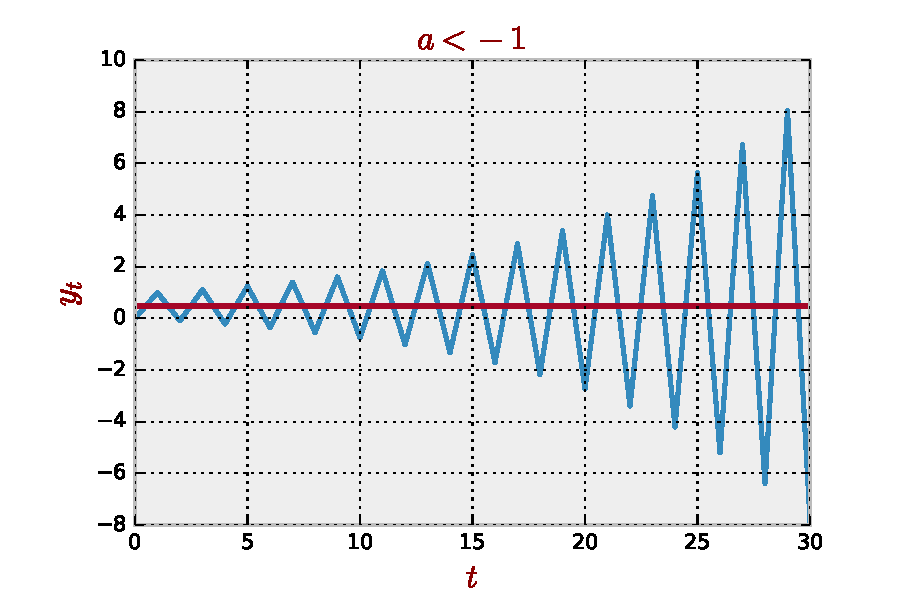
\includegraphics[scale=0.3]{./figs/fig1} & 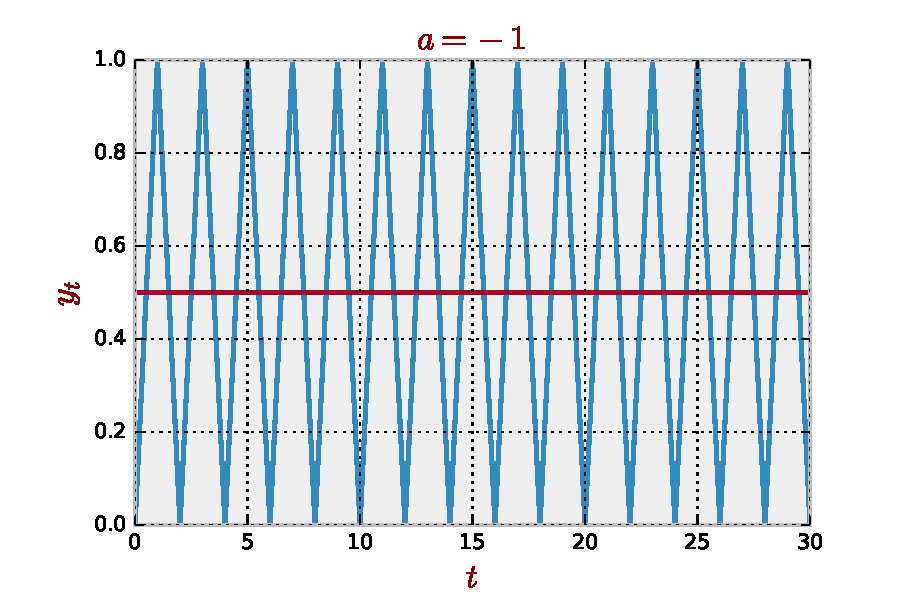
\includegraphics[scale=0.3]{./figs/fig2}\\
		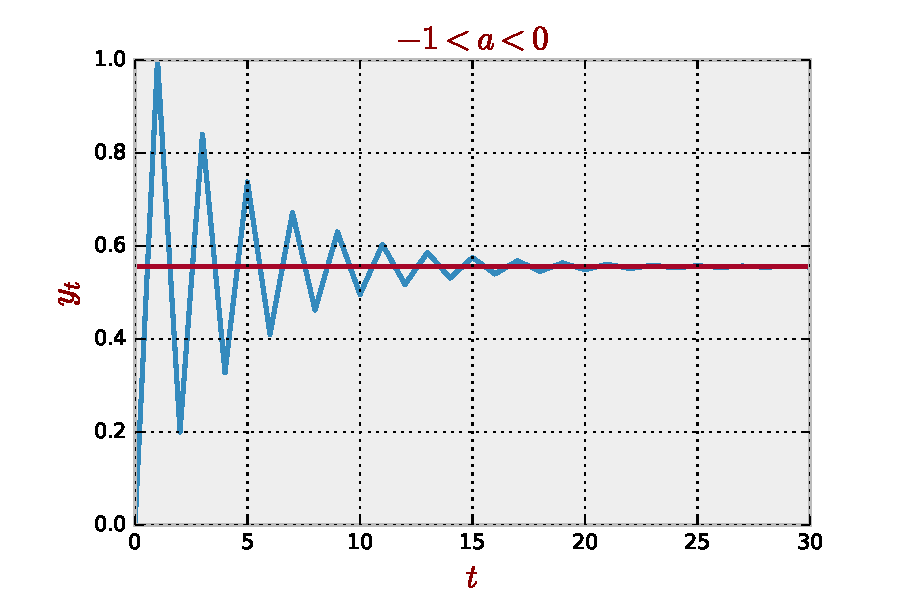
\includegraphics[scale=0.3]{./figs/fig3} & 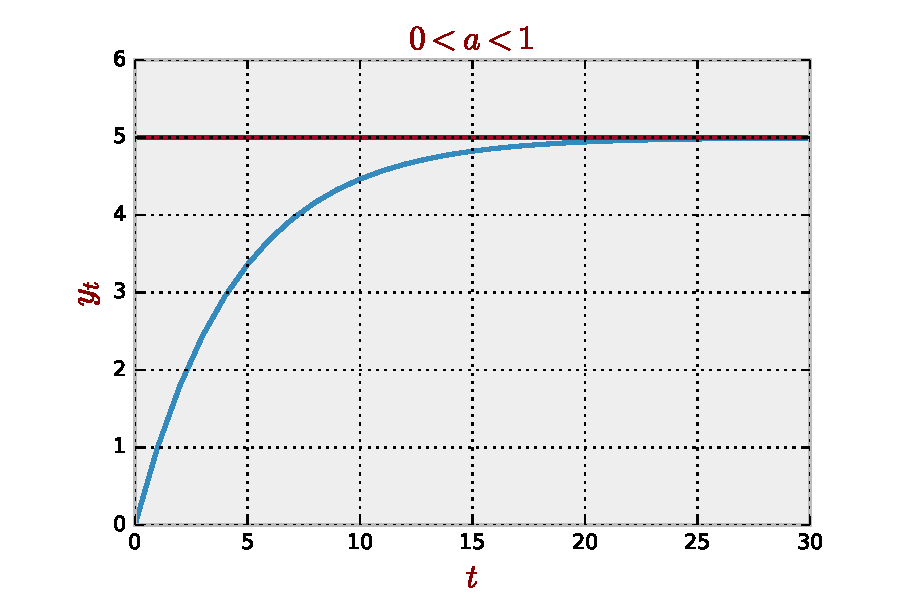
\includegraphics[scale=0.3]{./figs/fig4}
\end{tabular}

\end{center}
\end{frame}

\begin{frame}[fragile]
\frametitle{Fixed-point Stability (3)}
\begin{center}
	\begin{tabular}{cc}
		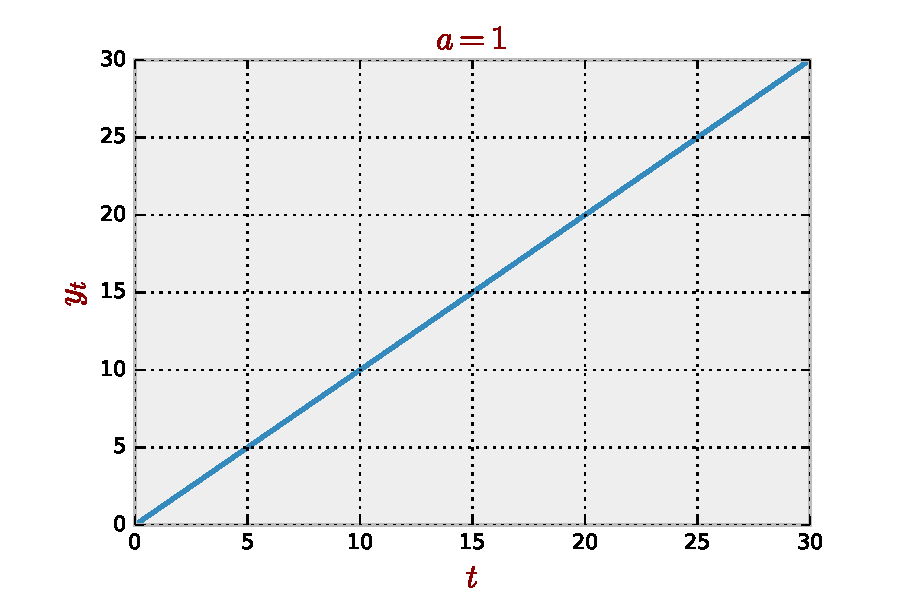
\includegraphics[scale=0.3]{./figs/fig5} & 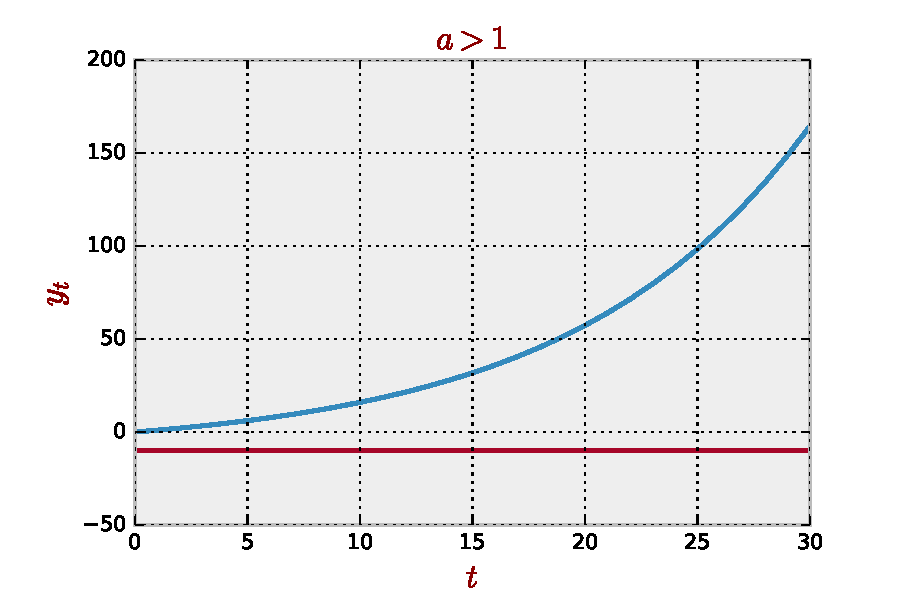
\includegraphics[scale=0.3]{./figs/fig6}
\end{tabular}

\end{center}
\end{frame}

\begin{frame}[fragile]
\frametitle{Time-varying $b$}
\begin{itemize}
	\item Let $b_{t}$ be an arbitrary but known function of $t$ (i.e. the values of $b_{t}$ are given beforehand)
	\item The equation becomes:
	\[
		y_{t+1} = ay_{t} + b_{t}, \quad t = 0,1,2,\ldots
	\]
	\item Starting from a given $y_{0}$, recursive substitutions leads eventually to:
	\[
		y_{t} = a^{t}y_{0} + \sum_{k=0}^{t-1}a^{t-k-1}b_{k}, \quad t = 0,1,2,\ldots
	\]
	\item Fixed points and stability conditions are much harder to specify
	\item However, equations of this kind are successfully used to describe special types of time series data (we'll get to this next semester)
	\item Stability conditions are derived after plausible assumptions on $b_{t}$ are made
\end{itemize}
\end{frame}

\begin{frame}[fragile]
\frametitle{Time-varying $a$}
\begin{itemize}
	\item If, in addition to $b$, the coefficient $a$ also changes over time, then the equation becomes:
	\[
		y_{t+1} = a_{t}y_{t} + b_{t}, \quad t = 0,1,2,\ldots
	\]
	\item The same line of reasoning as before can be applied finally leading to:
	\[
		y_{t} = \left(\prod_{k=0}^{t-1}a_{k}\right)y_{0} + \sum_{i=0}^{t-1}\left(\prod_{k=i+1}^{t-1}a_{k}\right)b_{i}
	\]
	where all terms $\displaystyle \prod_{k=t}^{t-1}a_{k}$ are set to equal 1.
\end{itemize}
\end{frame}

\begin{frame}[fragile]
\frametitle{Example 1: Mortgage Repayment}
\begin{itemize}
	\item An amount equal to $K$ is borrowed at time 0 to finance a mortgage at the fixed monthly interest rate $r$
	\item The mortgage is repaid monthly at amounts equal to $a$, and the number of monthly payments until full repayment equals $T$
	\item In each period the outstanding principal $b_{t}$ satisfies the following relationship:
	\[
		b_{t+1} = (1+r)b_{t} - a
	\]
	\item Additionally, it is obvious from the problem that $b_{0} = K$ and $b_{T} = 0$ 
\end{itemize}
\end{frame}

\begin{frame}[fragile]
\frametitle{Example 1: Mortgage Repayment (2)}
\begin{itemize}
	\item Assuming that $r > 0$, the fixed point is:
	\[
		b^{*} = -\frac{a}{1 - (1+r)} = \frac{a}{r}
	\]
	\item Therefore, the solution is:
	\[
		b_{t} = (1+r)^{t}\left(b_{0} - \frac{a}{r}\right) + \frac{a}{r}
	\]
	or:
	\[
		b_{t} = (1+r)^{t}\left(K - \frac{a}{r}\right) + \frac{a}{r}
	\]
\end{itemize}
\end{frame}

\begin{frame}[fragile]
\frametitle{Example 1: Mortgage Repayment (3)}
\begin{itemize}
	\item For $t=T$, the solution is:
	\[
		0 = (1+r)^{T}\left(K - \frac{a}{r}\right) + \frac{a}{r}
	\]
	\item If we solve the latter for $K$, we get:
	\[
		K = \frac{a}{r}\left(1 - \frac{1}{(1+r)^{T}}\right) = a\sum_{t=1}^{T}\frac{1}{(1+r)^{t}}
	\]
	i.e. the borrowed amount equals the sum of PDVs of all monthly payments until full repayment
\end{itemize}
\end{frame}

\begin{frame}[fragile]
\frametitle{Example 1: Mortgage Repayment (4)}
\begin{itemize}
	\item We could also solve for $a$:
	\[
		a = \frac{rK}{1 - (1+r)^{-T}} = \frac{rK(1+r)^{T}}{(1+r)^{T} - 1}
	\]
	or, in other words, this result allows to calculate the monthly mortgage payment given the borrowed amount and the interest rate
\end{itemize}
\end{frame}

\begin{frame}[fragile]
\frametitle{Example 2: Compound Interest and PDVs with Constant Interest Rates}
\begin{itemize}
	\item Let $w_{t}$ denote a person's wealth (assets) at time $t$
	\item If $y_{t}$ and $c_{t}$ are respectively this person's income and consumption
	\item Given a constant interest rate $r$, we have:
	\[
		w_{t+1} = (1+r)w_{t} + y_{t+1} - c_{t+1}
	\]
	\item If initial wealth is $w_{0}$, then the solution is:
	\[
		w_{t} = (1+r)^{t}w_{0} + \sum_{k=0}^{t-1}(1+r)^{t-k-1}(y_{k+1} - c_{k+1})
	\]
\end{itemize}
\end{frame}


\begin{frame}[fragile]
\frametitle{Example 2: Compound Interest and PDVs with Constant Interest Rates (2)}
\begin{itemize}
	\item Divide both sides by $(1 + r)^{t}$ to get:
	\[
		(1+r)^{-t}w_{t} = w_{0} + \sum_{k=0}^{t-1}(1+r)^{-k-1}(y_{k+1} - c_{k+1})
	\]
	\item The left-hand side is the PDV of $w_{t}$ at time 0
	\item It equals the initial wealth plus the PDV of the flow of savings from time 1 to time $t$
\end{itemize}
\end{frame}

\begin{frame}[fragile]
\frametitle{Example 3: The Harrod-Domar Growth Model}
\begin{itemize}
	\item We consider the discrete-time version
	\item Saving is a fixed share of output/income:
	\[
		S_{t} = s Y_{t},\quad 0 < s < 1
	\]
	\item Investment depends on output growth:
	\[
		I_{t} = v(Y_{t} - Y_{t-1}), \quad v > 0
	\]
	\item Saving equals investment:
	\[
		S_{t} = I_{t}
	\]
\end{itemize}
\end{frame}

\begin{frame}[fragile]
\frametitle{Example 3: The Harrod-Domar Growth Model (2)}
\begin{itemize}
	\item Substituting the first two equations into the third yields:
	\[
		sY_{t} = v(Y_{t} - Y_{t-1}) \Rightarrow Y_{t} = \frac{v}{v-s}Y_{t-1}
	\]
	\item Solving the equation leads to:
	\[
		Y_{t} = \left(\frac{v}{v-s}\right)^{t}Y_{0},
	\]
	and the only fixed point is 0
	\item There are several possibilities for the relationship between $s$ and $v$, leading to different conclusions on the stability of the system
\end{itemize}
\end{frame}

\begin{frame}[fragile]
\frametitle{Example 4: Hog Cycles and Cobwebs}
\begin{itemize}
	\item Based on the fact that for various commodities output and prices exhibit cyclical behaviour  
	\item Cycles stem from the consecutive adjustments, which are manifested as movements between the supply and demand curve
	\item Also, from the technological perspective, there is a span of time required in order to produce a certain output (e.g. in agriculture)
	\item Generally speaking, the ``cobweb phenomenon'' stems from the presence of lagged effects on some economic variables
	\item Also, there is a mismatch between the time of the production decision and the time of purchase decisions by customers (demand)
\end{itemize}
\end{frame}

\begin{frame}[fragile]
\frametitle{Example 4: Hog Cycles and Cobwebs (2)}
\begin{itemize}
	\item Initially, the system (the market) is in equilibrium
	\item Each cycle begins with a demand or with a supply shock
	\item In this version of the model, only one-period lags matter
	\item Supply, demand, and equilibrium are described via the following three equations:
	\[
	\begin{array}{lcl}
		q_{t}^{D} = \alpha - \beta p_{t}\\
		\quad\\
		q_{t}^{S} = \gamma + \delta p_{t-1}\\
		\quad\\
		q_{t}^{D} \equiv q_{t}^{S}
	\end{array}
	\]
	
	where $\alpha > 0, \beta > 0$, and $\delta > 0$.
\end{itemize}
\end{frame}

\begin{frame}[fragile]
\frametitle{Example 4: Hog Cycles and Cobwebs (3)}
\begin{itemize}
	\item Substituting supply and demand in the equilibrium condition leads to the following difference equation:
	\[
		p_{t} = \frac{\alpha - \gamma}{\beta} - \frac{\delta}{\beta}p_{t-1},
	\]
	\item Its solution is:
	\[
		p_{t} - p^{*} = \left(-\frac{\delta}{\beta}\right)^{t}(p_{0} - p^{*})
	\]
	
	where $p^{*}$ is the equilibrium price
	\item There are three possible system behaviours depending on the values of $\delta$ and $\beta$
\end{itemize}
\end{frame}

\begin{frame}[fragile]
\frametitle{Example 4: Hog Cycles and Cobwebs (4)}
\begin{center}
	\begin{tabular}{ccc}
		\includegraphics[scale=0.3]{./figs/fig7} & 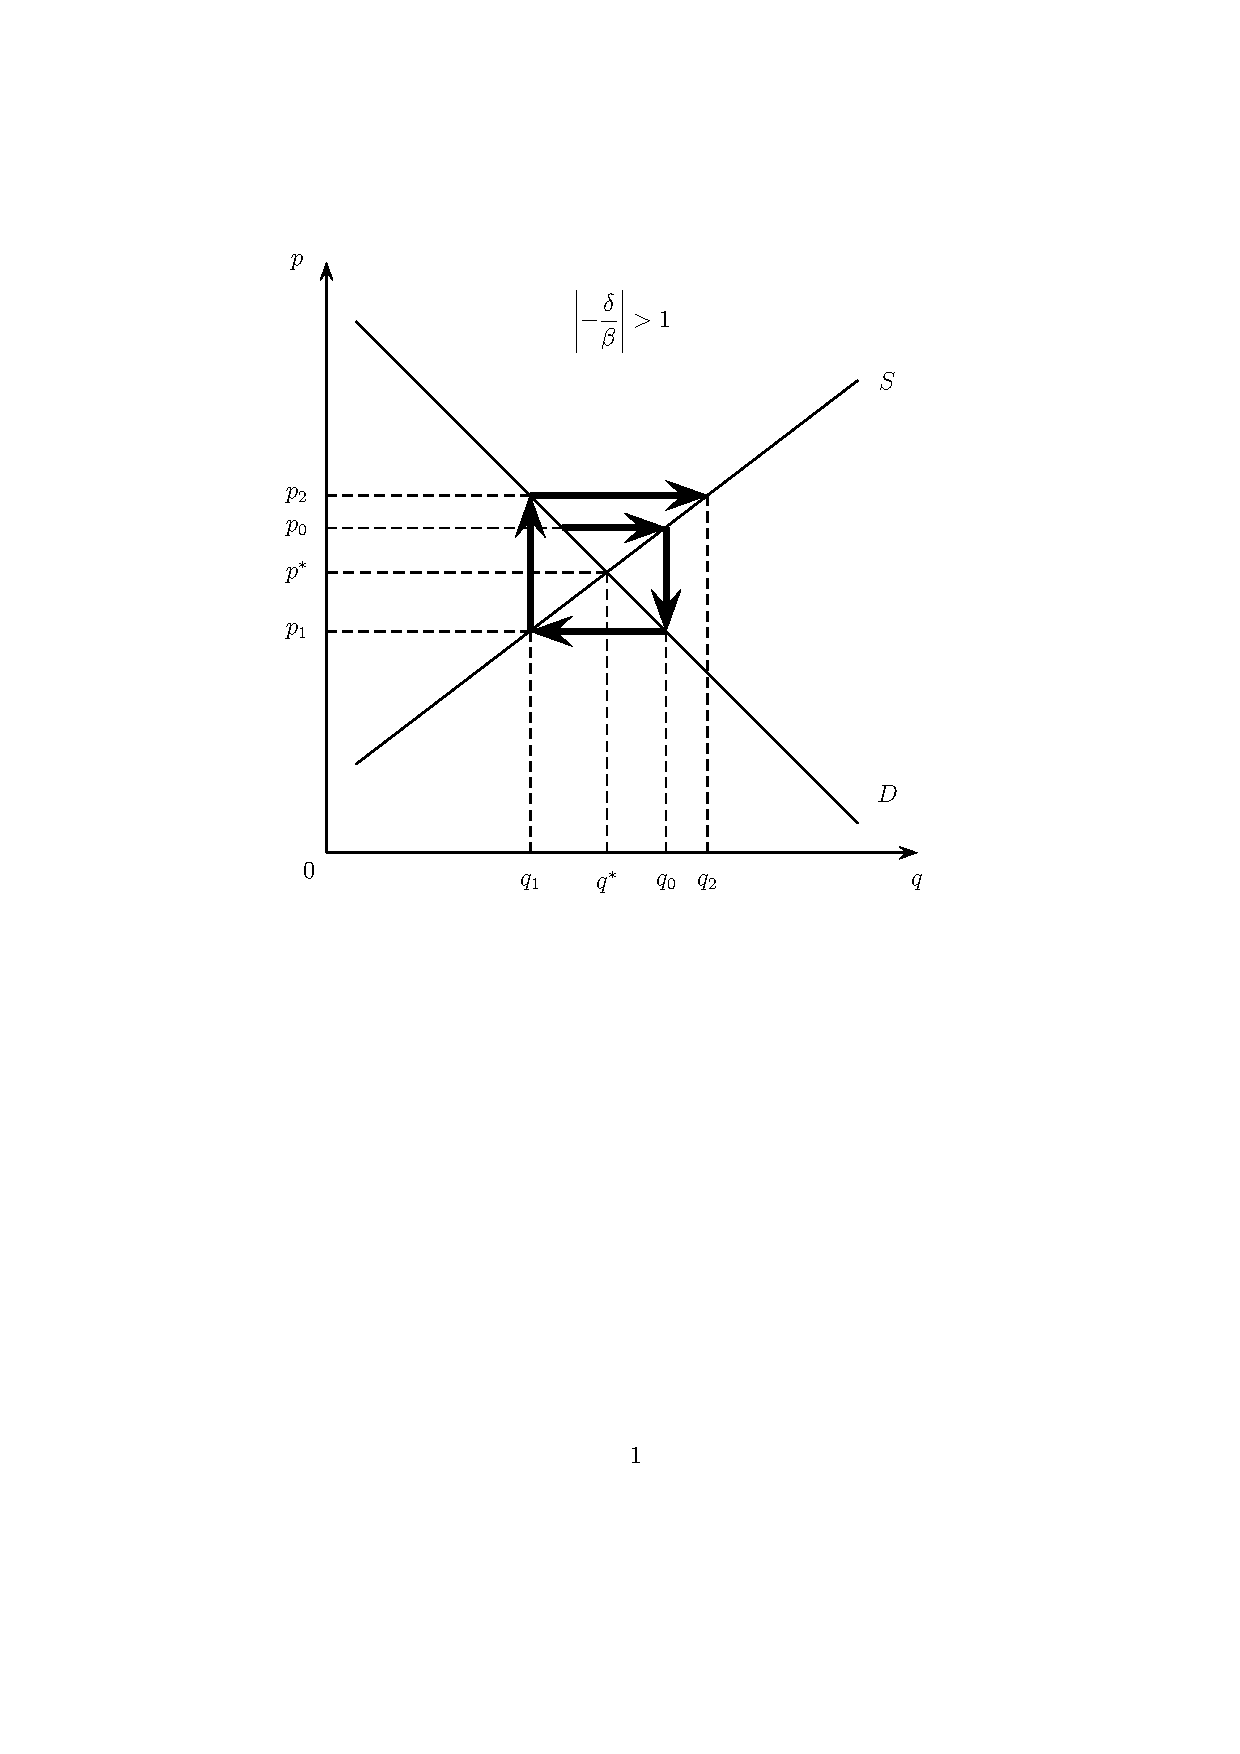
\includegraphics[scale=0.3]{./figs/fig8} & 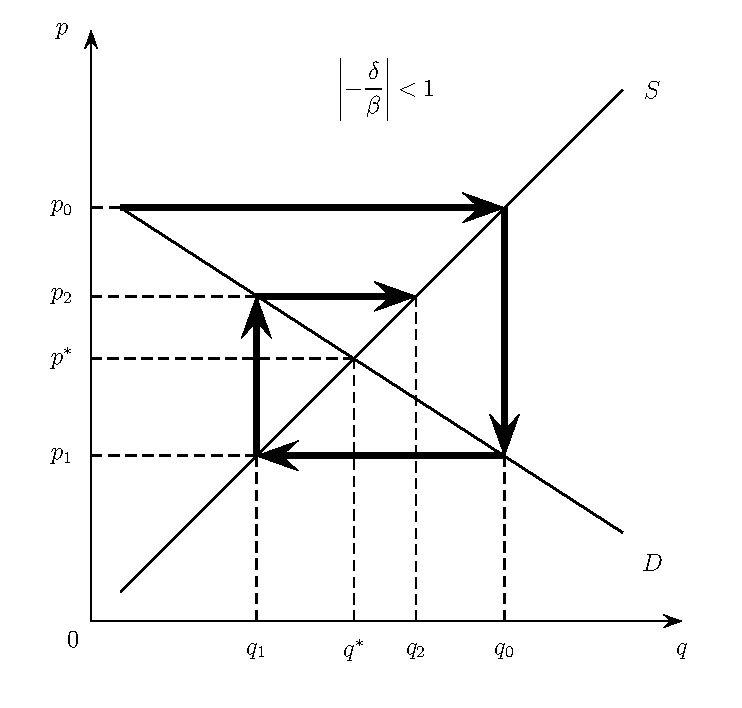
\includegraphics[scale=0.3]{./figs/fig9}
	\end{tabular}
\end{center}
\end{frame}

\begin{frame}[fragile]
	\frametitle{References}
	\begin{itemize}
		\item Syds{\ae}ter et al. (2008), ch. 11
		
		\item Chiang and Wainwright (2005), ch. 17
		
		\item Shone (2002), ch. 3
	\end{itemize}
\end{frame}
\end{document}
	


